%----------------------------------------------------------------------------
%               Template for OOPSLA
%               based on:
%               Template for sigplanconf LaTeX Class
%
% Name:         sigplanconf-template.tex
%
% Purpose:      A template for sigplanconf.cls, which is a LaTeX 2e class
%               file for SIGPLAN conference proceedings.
%
% Guide:        Refer to "Author's Guide to the ACM SIGPLAN Class,"
%               sigplanconf-guide.pdf
%
% Author:       Paul C. Anagnostopoulos
%               Windfall Software
%               978 371-2316
%               paul@windfall.com
%
% Created:      15 February 2005
%
%-----------------------------------------------------------------------------


\documentclass[11pt,numbers]{sigplanconf}
\usepackage[final]{oopsla2016}

% The following oopsla2016 options are available:
%
% 1stsubmission   For the initial submission
% 2ndsubmission   For the 2nd submission
% final           For camera-ready

\usepackage{amsmath, array}
%\usepackage{mathpartir}
\usepackage{xcolor}
\usepackage{amsfonts}
\usepackage{amsthm}
\usepackage{listings}
\usepackage{xspace}
\usepackage{hyperref} 
\usepackage{floatrow}
\usepackage{subcaption}
\usepackage{graphicx, placeins, dblfloatfix, fixltx2e}
\usepackage[inline]{enumitem}


\newtheorem{theorem}{Theorem}
\newtheorem{lemma}{Lemma}
\newtheorem{definition}{Definition}
\theoremstyle{definition}
\newtheorem{exmp}{Example}[section]
\newtheorem{corollary}{Corollary}[theorem]

\newcommand{\eth}[0]{Ethereum}
\renewcommand{\sectionautorefname}{Section}
\renewcommand*{\bibfont}{\raggedright}
%\newenvironment{ppl}{\fontfamily{qcr}\selectfont}{\par}

% \DeclareCaptionFormat{myformat}{#1#2#3\hrulefill}
% \captionsetup[figure*]{format=myformat}


%\input{macros}

%aggressive tightening of lists.
\setlist{noitemsep}%\setlist{nosep}

\newenvironment{DIFnomarkup}{}{}
\begin{document}

\allowdisplaybreaks[1]

%\copyrightdata{978-1-nnnn-nnnn-n/yy/mm} 
%\doi{nnnnnnn.nnnnnnn}

% Uncomment one of the following two, if you are not going for the 
% traditional copyright transfer agreement.

%\exclusivelicense                % ACM gets exclusive license to publish, 
                                  % you retain copyright

%\permissiontopublish             % ACM gets nonexclusive license to publish
                                  % (paid open-access papers, 
                                  % short abstracts)
%\publicationrights{licensed}

\title{Ethereum Blockchain Compression}
\authorinfo{Anitha Gollamudi \and Yihe Huang}{Harvard University, Cambridge, MA, USA}{agollamudi@g.harvard.edu \and yihehuang@g.harvard.edu}
\maketitle
\begin{abstract}
Blockchain scalability is a well-known issue in the cryptocurrency community.
Clients have to download and store giga bytes of data to be able to mine and verify the transactions successfully.
In this work, we propose to compress the size of Ethereum blockchain by leveraging the structure of blocks and transactions.
A reduced blockchain can enable thin clients  that are constrained by storage and network bandwidth (e.g., IoT, embedded systems),
 to operate on the ethereum blockchain.


\end{abstract}


% % general terms are not compulsory anymore, 
% % you may leave them out
% \terms
% term1, term2

%\onecolumn
\section{Introduction} \label{sec:intro}

\eth{} is a public blockchain based cryptocurrency and supports Turing-complete smart contracts~\cite{ethereum}.
The blockchain maintains a list of records, called \emph{blocks} and serves as a ledger for all transactions.
The value token of the blockchain is called \emph{ether} and 
is traded in cryptocurrency exchanges.
Clients use ether to pay for executing and maintaining the transactions.~\footnote{
\emph{Finney}, \emph{Szabo}, and \emph{Wei} are the denominations of ether.}
There are two kinds of \eth{} accounts: 
\renewcommand\labelenumi{(\theenumi)}
\begin{enumerate*}
	\item \emph{Externally owned accounts} (EOA) and
	\item \emph{Contract accounts}.
\end{enumerate*}
Contract accounts are special accounts containing the smart contracts in bytecode format, referred to as \emph{EVM bytecode}.
The bytecode is stack-based and is executed on \emph{Ethereum Virtual Machine} (EVM).
Contract accounts comprise around $25\%$ of the entire \eth{} accounts.~\footnote{
At the time of writing, number of EOA and contract accounts are 555,043 and 197,261 respectively.}  
 
Currently there are around 2,488,503 blocks with size ranging between 1.5KB to 12.5KB~\cite{ethblocksize}.  
The blockchain is growing at a rate of 1.2GB/month and
the space required for storing full blockchain is as high as 60GB~\cite{ethdiskspace}.
Compressing the blockchain can therefore be useful for full client nodes (e.g., IoT, embedded systems with less storage)
that download the entire blockchain.

In this project, we propose to compress the entire \eth{} blockchain by leveraging the domain-specific information.
One could use the general-purpose compression software (e.g., gzip, bzip2, 7zip) and compress the blockchain.
However, a majority of blockchain contains 256-bit hashes which, if we assume are perfectly random, will be hard to compress.
Also these programs cannot exploit certain properties that are specific to blockchain and thus do not offer optimal outputs.
Our goal is to come-up with compression techniques that  are specialized for blockchain.
While we aim to provide a comparative study, we do not conjecture that our compression algorithm always outperforms the existing mature compressors.
We believe that the insights can be added as an extension to be able to get effective compression rates.   

Blockchain compression involves compressing each block.
Although compressing a block (and hence transactions) also includes compressing EVM bytecode, 
for the sake of exposition we view them as complementary tasks. 
In particular, techniques to compress bytecode are orthogonal to techniques for compressing other fields of transaction.
In Section~\ref{sec:blockcompress} and 
Section~\ref{sec:evmcompress}, we   
outline the opportunities for compressing \eth{} block and EVM bytecode. 

\subsection{Ethereum Block Compression}\label{sec:blockcompress}

A block is comprised of a block header, ommer (parent) block headers and a series of transactions. 
A block header stores cryptographic hashes of all transactions in the block as well as of previous and parent blocks.
These hashes play an important role for verifying the validity of blocks.
It might seem that there is not enough information to compress these random bits. 
The block hashes, however, have a fixed number of leading zeros and
can therefore be encoded more efficiently.
Also, a closer inspection at the block header reveals that 
some information is either redundant or can be computed given other fields of the block.
We explain how to exploit this redundancy to efficiently encode the block information.

A block header has the following format. We outline the possibility of efficiently encoding some fields. 
\begin{description}
 \item[parentHash] 
 \item[ommersHash:]  Keccak 256-bit hash.
 \item[stateRoot]  
 \item[transactionsRoot]
 \item[beneficiary:]160-bit address.
 \item[logsBloom:] Bloom filter for log entries.
 \item[difficulty:] Can be computed from previous block using the formula
 $$
 D_{c} = D_{p} + \dfrac{D_{p}}{2048\times\textrm{max}\left(\dfrac{1 - (ts_{c} - ts_{p})}{10}, -99\right)} + 2^{b/10^5-2}
 $$
 where $ts$ denotes timestamps, subscripts $c$ and $p$ denote current and parent blocks respectively, and $b$ is the block number.
 This suggests the possibility of saving bits without having to store difficulty for all blocks.
 \item[number:] Number of ancestor blocks
 \item[gasLimit:] Scalar value limiting the gas expenditure
 \item[gasUsed:] Scalar value indicating the total gas used by all transactions in the block. This information can encoded efficiently.
 \item[timestamp]
 \item[extraData]
 \item[mixHash:] 256-bit hash
 \item[nonce:] 64-bit hash
\end{description}

An efficient encoder can exploit that \textbf{difficulty} and \textbf{gasUsed} can computed on the fly and therefore save around 512 bits of information per block (Recall that \eth{} uses 256-bit integers by default).  


A transaction is a signed message. 
Transactions are much more compressible and can be a major source of compression gains.
There are two types of transactions: {\em Contract Creation} transactions and {\em Message Call} transactions.
Both types have the following common fields:
\begin{description}
  \item[nonce:] A scalar value representing number of transactions associated with this account
  \item[gasPrice:] Default value is $0.02\times10^{12}$ Wei. Though clients can set their own gasPrice, most of the transactions use default value suggesting the high probability of its occurance.
  \item[gasLimit:] Maximum gas that can be used for executing this transaction
  \item[to:] Receiver's 160-bit address. For contract creation, a special symbol $\phi$ is used.
  \item[value:] Wei being transferred to the recipient.
  \item[v,r,s:] v =\{27, 28\} and so can be efficiently encoded.
\end{description}

Additionally, a Contract Creation transaction has an \textbf{init} field containing the EVM bytecode for initializing the contract.
We propose to compress the EVM bytecode using techniques presented in Section~\ref{sec:evmcompress}.

A Message Call transaction has \textbf{data} field that contains the inputs of the message call: a method ID and parameters supplied to the invoked method.
Existing transactions suggest that most of the inputs are going to a high number of 0's~\cite{ethtx}. 
This is because \eth{} uses 256-bit big integers, but most of the transactions limit themselves to using 64-bit integers.
This suggests that small numbers can be encoded efficiently.


%
\subsection{EVM ByteCode Compression}\label{sec:evmcompress}

There are several ways to compress EVM bytecode. Huffman encoding is probably the most straightforward
way to reduce bytecode size. By using Huffman encoding, we essentially compress instructions individually
by minimizing the number of bits taken by each opcode given how frequently they appear. One potential
benefit of using Huffman codes is that we can modify the EVM to directly execute the compressed bytecode,
without decoding the entire bytecode stream first. It, however, raises the challenge of making program counter modifications work
correctly, because now instructions are variable-length encoded.

Huffman codes reduce the size of individual instruction encoding, but do not take advantage of repetitive patterns in the bytecode.
A dictionary-based or grammar-based compression scheme can further reduce redundant information in the bytecode.
General-purpose compression algorithms like the LZ-family or Sequitur might just work,
but likely not optimal, because of the specific structure in bytecode sequences.
For example, some instructions take operands, sometimes very long operands.
Long operands are usually just random bits and are much harder to compress than the opcodes, which typically appear in patterns.
These long operands may confuse general-purpose compress algorithms, resulting in sub-optimal results.
We aim to devise a domain-specific compression scheme for EVM bytecode that can achieve better compression rates
by treating operands the opcodes separately.



%
\subsection{EVM ByteCode Compression}\label{sec:evmcompress}

There are several ways to compress EVM bytecode. Huffman encoding is probably the most straightforward
way to reduce bytecode size. By using Huffman encoding, we essentially compress instructions individually
by minimizing the number of bits taken by each opcode given how frequently they appear. One potential
benefit of using Huffman codes is that we can modify the EVM to directly execute the compressed bytecode,
without decoding the entire bytecode stream first. It, however, raises the challenge of making program counter modifications work
correctly, because now instructions are variable-length encoded.

Huffman codes reduce the size of individual instruction encoding, but do not take advantage of repetitive patterns in the bytecode.
A dictionary-based or grammar-based compression scheme can further reduce redundant information in the bytecode.
General-purpose compression algorithms like the LZ-family or Sequitur might just work,
but likely not optimal, because of the specific structure in bytecode sequences.
For example, some instructions take operands, sometimes very long operands.
Long operands are usually just random bits and are much harder to compress than the opcodes, which typically appear in patterns.
These long operands may confuse general-purpose compress algorithms, resulting in sub-optimal results.
We aim to devise a domain-specific compression scheme for EVM bytecode that can achieve better compression rates
by treating operands the opcodes separately.


\section{Methodology Overview}\label{sec:overview}
In this section we describe the necessary technical details about \eth{}'s implementation, and how we exploit them for compression.
We decided to work with the \eth{} blockchain export format.
The format is standard among all \eth{} clients and can be used for backup/restore purposes.

The exported blockchain file is a simple concatenation of a series of blocks.
Each block contains a header and a list of transactions included in the block.
Each \eth{} block also include a list of {\em uncles}, which are special parent blocks not part of the main chain.
Uncles are specific to \eth{} to encourage mining while accounting for the blockchain's short block time.
We now explain each of these components and discuss compression opportunities in more detail.

%A block is comprised of a block header, ommer (parent) block headers and a series of transactions. 
%A block header stores cryptographic hashes of all transactions in the block as well as of previous and parent blocks.
%These hashes play an important role for verifying the validity of blocks.
%It might seem that there is not enough information to compress these random bits. 
%The block hashes, however, have a fixed number of leading zeros and
%can therefore be encoded more efficiently.
%Also, a closer inspection at the block header reveals that
%some information is either redundant or can be computed given other fields of the block.
%We explain how to exploit this redundancy to efficiently encode the block information.

\subsection{Block Header}
The block header is the metadata portion of an \eth{} block. The block header contain important
information about the content of the block, and the hash of the header is usually regarded as the ``block hash''
used in proof-of-work validation.
Block headers have the following format:

\begin{table}[H]
	\centering
\begin{tabular}{>{\bfseries}l c l}
 parentHash&:& Hash of the previous block in the main chain\\
 uncleHash&:& Hash of the list of uncles\\
 stateRoot&:& Merkle-tree root for fast verification of transactions\\
 transactionsRoot&:& Hash of the list of transactions\\
 coinbase&:& Address to which the coinbase reward (mining reward) is paid to\\
 logsBloom&:& Bloom filter for log entries\\
 difficulty&:& Proof-of-work difficulty of this block\\
 number&:& Height of this block\\
 gasLimit&:& Scalar value limiting the gas expenditure\\
 gasUsed&:& Scalar value indicating the total gas used by all transactions in the block\\
 timestamp&:&\\
 extraData&:&\\
 mixHash&:& Special hash for fast verification of block difficulty\\
 nonce&:& The proof of work\\
\end{tabular}
\end{table}

The block header contains many redundant information and therefore presents opportunities for efficient encoding.
The \textbf{difficulty} field, for exmaple, can be computed using the following equation according to~\cite{ethereum}.

$$
D_{c} = D_{p} + \dfrac{D_{p}}{2^{11}\cdot\max\left(\dfrac{1 - (ts_{c} - ts_{p})}{10}, -99\right)} + 2^{b/10^5-2}
$$

where $ts$ denotes timestamps, subscripts $c$ and $p$ denote current and parent blocks respectively, and $b$ is the block number.
This suggests that we don't have to store difficulty in the block headers.
Fields like \textbf{transactionsRoot} and \textbf{parentHash} are also redundant.
\textbf{transactionsRoot} can be deterministically computed from the list of transactions included in the block,
and \textbf{parentHash} can be reconstructed by locating the parent block by block height and re-hashing the header.

\textbf{logsBloom} is a Bloom filter used as a digest of all logs generated by transactions.
It is used to validate the logging behavior of smart contract transactions. The Bloom filter occupies 256 bytes,
but according to our observation most of the bytes are zero. This again presents opportunities for compression.
In our implementation, we used run-length encoding to encode such zero bytes in the Bloom filter.

\subsection{Transaction}

A transaction is a signed message indicating some action like account transfer or contract execution.
Transactions are much more compressible and can be a major source of compression gains.
Each transaction has the following format:

\begin{table}[H]
	\centering
	\begin{tabular}{>{\bfseries}l c p{0.8\textwidth}}
  nonce&:& A scalar value representing number of transactions associated with this account\\
	gasPrice&:& \par{Default value is $0.02\times10^{12}$ Wei. Though clients can set their own gasPrice, most of the transactions use default value suggesting the high probability of its occurance} \\
  gasLimit&:& Maximum gas that can be used for executing this transaction\\
  to&:& Receiver's 160-bit address. The address is empty for contract creation.\\
  payload&:& Additional data for contract-related transactions\\
  value&:& Wei being transferred to the recipient. For contract-related transactions, this field is zero.\\
  v, r, s&:& Cryptographic signature of the transaction\\
\end{tabular}
\end{table}

The \textbf{payload} field contains EVM bytecode as well as message call data for contract-related transactions,
both are highly compressable. We decided to use Huffman encoding to reduce the footprint of EVM bytecode,
and apply the more sophiscated gzip compression on top of that.
For message call transactions, the \textbf{payload} field contains message call data that represent a method ID and
parameters supplied to the contract method being invoked.
Message call data have a large number of zero bytes, because \eth{} uses 256-bit integers,
while most smart contract still only use the lower 64 bits.
We also use run-length encoding to encode the repeating zero bytes in message call data.
%Additionally, a Contract Creation transaction has an \textbf{init} field containing the EVM bytecode for initializing the contract.
%We propose to compress the EVM bytecode using techniques presented in Section~\ref{sec:evmcompress}.
%A Message Call transaction has \textbf{data} field that contains the inputs of the message call: a method ID and parameters supplied to the invoked method.
%Existing transactions suggest that most of the inputs are going to have a high number of 0's~\cite{ethtx}. 
%This is because \eth{} uses 256-bit big integers, but most of the transactions limit themselves to using 64-bit integers.
%This suggests that small numbers can be encoded efficiently.

\subsection{Other Considerations}

We decided not to apply any special treatment to uncles due to their rareness in the blockchain.

We also note the additional compression opportunities by reorganizing the blockchain.
We propose to reorganize the blockchain by grouping blocks according to their coinbase reward addresses.
Due to effects of pooled mining, most blocks are mined by a relatively small number of mining pools.
This means that a large number blocks can potentially have the same coinbase reward address.
Reorganizing the blocks by coinbase reward addresses avoid repeating such information in each block.
Within each block, we also propose to organize transactions by their recipient addresses, so that
transactions to the same address will only have the recipient address written in the block once.

We also studied the possibility of grouping transactions by their ``from'' addresses.
Unfortunately the ``from'' address is encoded in the signature, and it's impossible to
separate signatures from individual transactions.


\section{Implementation}\label{sec:implement}
We implemented our compression scheme as an extension to go-ethereum client.


\section{Evaluation}\label{sec:evaluation}

We evaluate our custom compression scheme against Morden, Ropsten and Frontier blockchains.
Our approach is two-fold:
\begin{enumerate*}
	\item We first transform the exported blockchain to our custom format and compare the gains in savings
	\item We then compress the custom formatted blockchain using traditional compression programs (gzip, bzip2 and xz) and compare the savings obtained by compressing the exported i.e., original blockchain.
\end{enumerate*}
Our evaluation approach enables us to guage the additional gains that are possible by extending the traditional compression programs with blockchain compression feature. 
We only present the evaluation results in this section and 
postpone the further discussion until~\autoref{sec:discuss}. 

\paragraph{Ropsten}
Ropsten is the latest private blockchain aimed as a testnet for the \eth{} developers. It was launched recently and therefore has fewer transactions but characterizes the main blockchain fairly well.\footnote{Launched on Nov 20, 2016.}
It has about 120K blocks and 170K transactions of which 8.5K (about 5\%) create new contracts.
Occupying a size of about 100MB, this is the smallest blockchain in our evaluation. 
\paragraph{Frontier}
Frontier is the main \eth{} blockchain and occupies around 3.5GB. It has 3M blocks and 13M transactions of which 225K (about 1.7\%) create transactions. 
This is the largest blockchain in our evaluation.

\paragraph{Morden}
Morden is a private blockchain serving as a testnet since the start of \eth{} blockchain. 
It has about 1.9M blocks and 5M transactions of which 108K (about 2 \%) create new contracts. The entire blockchain occupies about 2.1GB.

\newfloatcommand{capbtabbox}{table}[][\FBwidth]
\begin{figure}[!t]
\CenterFloatBoxes
\begin{floatrow}
\capbtabbox{
	\begin{tabular}{ >{\bfseries}c| p{1.5cm} | p{1.5cm} | p{1.5cm} |p{1.5cm}}
	Blockchain& {Size of Original File (MB)} & {\par{Size of Custom format without Huffman Encoding (MB)}} & {Size of Custom format with Huffman Encoding (MB)} \\
  \hline
  Ropsten & 98.6 & 47.8  & 44.4 \\
  Morden & 2160 & 1135.4 &1068.9  \\
  Frontier  & 3434.6  & 2069 & 2037.5 \\ 
\end{tabular}
%\begin{tabular}{ >{\bfseries}c| p{1.5cm} | p{1.5cm} | p{1.5cm} |p{1.5cm} |p{1.5cm} }
%	Blockchain& {Size of Original File (MB)} & {\par{Size of Custom format \newline (MB)}} & {Size of Custom format with Huffman Encoding (MB)} & \par{Percentage Gain without Huffman Encoding}  & \par{Percentage Gain with Huffman Encoding} \\
%  \hline
%  Ropsten & 98.6 & 47.8  & 44.4 &51.5  & 55.0\\
%  Morden & 2160 & 1135.4 &1068.9 & 47.4 & 50.5 \\
%  Frontier  & 3434.6  & 2069 & 2037.5 & 39.6 & 40.7\\
%\end{tabular}
}{
\caption{Compression using our custom format with and without Huffman encoding} 
\label{tab:origvscustom}
}
\ffigbox{
	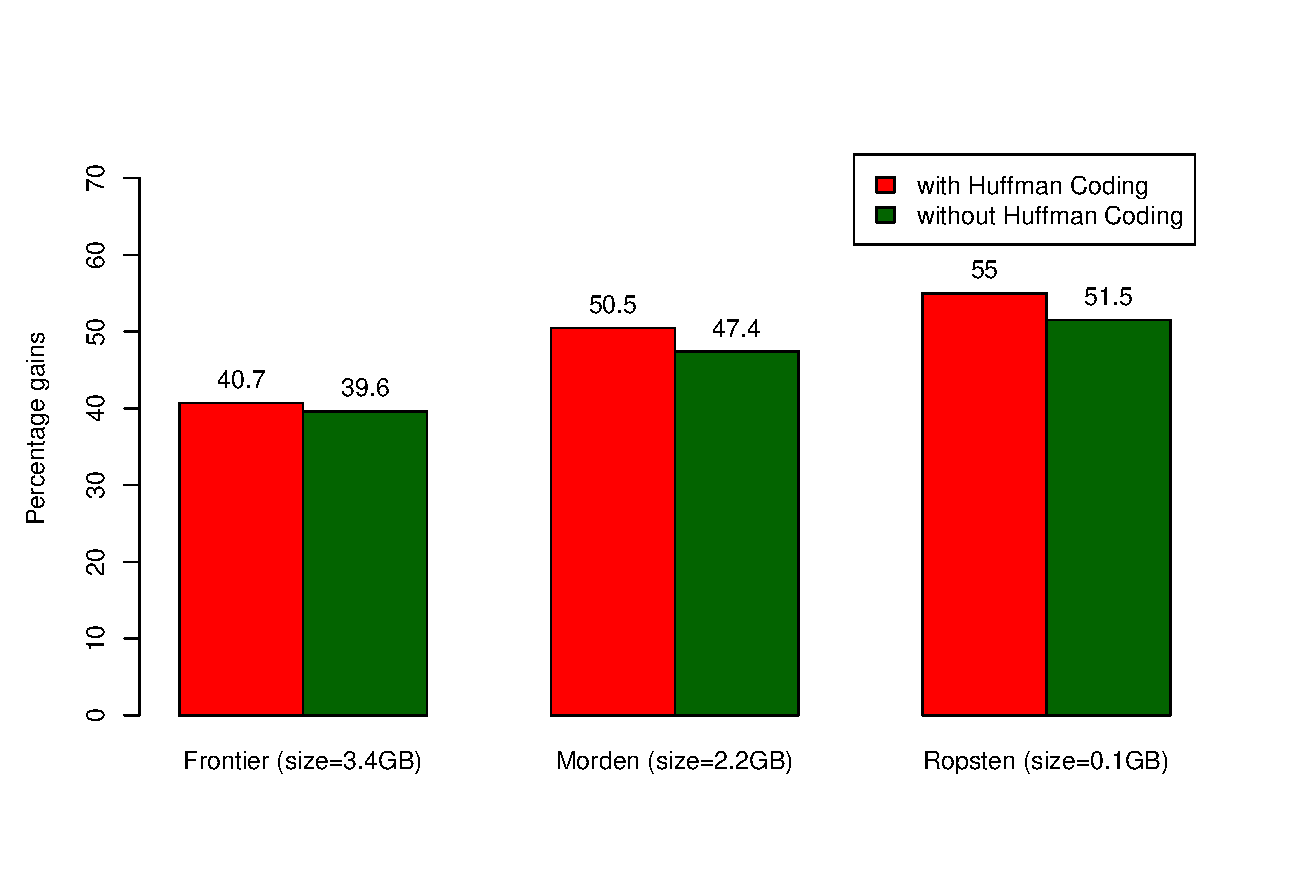
\includegraphics[scale=0.39]{plots/customgains.eps}
	%\rule{3cm}{3cm}
}{ \caption{Percentage gains}
\label{fig:origvscustom}
}
\end{floatrow}
\end{figure}

\FloatBarrier
Table~\ref{tab:origvscustom} shows the size of the blockchains before and after applying our technique. Third and fourth columns show the impact of assigning Huffman codes to EVM opcodes. 
As expected, using Huffman codes lead to further savings because frequently
used opcodes now use fewer bits.
\autoref{fig:origvscustom} shows the percentage gain in space savings due to our technique. This is a standard computation:
\[ 
	\text{percentage gain} = \big ( 1 - \frac{\text{size of custom formatted blockchain}}{\text{size of original blockchain}}\big ) \times 100
\]
Savings are greater when Huffman code are assigned and are as high as $55\%$ for Ropsten. Even on Frontier blockchain, $40\%$ space savings can be observed demonstrating the usefulness of our technique. 
Interestingly, Huffman codes did not bring about lot of savings for Frontier ($\sim1\%$) though they result in about $3\%$ additional savings in Morden and Ropsten networks.
We attribute this to two possibilities:
\begin{enumerate*}
	\item Our Huffman code assignment uses the opcode frequency distribution from Morden network. The Frontier network may have a slightly different distribution.
	\item EVM bytecode constitutes about $13\%$ of the Morden blockchain  but only $8\%$ of the frontier blockchain. 
		This is probably not a huge difference, but could contribute to smaller savings.
\end{enumerate*}

As mentioned earlier, we do not aim to compete against the existing mature compression tools.
However, we provide a comparative evaluation of our tool against gzip, bzip2 and xz. 
These programs are tuned for best compression savings, i.e., \emph{gzip -9}, \emph{bzip2 -9} and \emph{xz -9} have been used. 
Note that the options are only tuned for getting best space savings and may result in increased compression times.
This is a reasonable trade-off given that our primary objective is to get best compression savings in terms of space.
We also evaluate the compression times to ensure that they are not
prohibitively longer.

\begin{table}[H]
\centering
\captionsetup{justification=centering}
\begin{tabular}{ >{\bfseries}c| p{2cm} | p{2cm} |p{2cm} | p{1.5cm} | p{1.5cm} }
	Program & {Compressed Size of Original File (MB)} & {Compressed Size on Custom format (MB)} & {Compressed Size on Custom format with Huffman Encoding (MB)}& Percentage Gain without Huffman Encoding & Percentage Gain with Huffman Encoding\\
  \hline
  gzip  & 33.4 & 27.5 & 29.4 & 17.7 & 12.0 \\
  bzip2 & 31.0 & 26.7 & 28.6 & 13.9 & 7.8  \\
  xz   & 27.8 & 22.4 &  23.3 & 19.4 & 16.2 \\
\end{tabular}
\caption{Compression of Ropsten testnet. \\ Original Size = 98.6MB. Custom format size = 47.8MB}
\label{tab:compropsten}
\end{table}
\autoref{tab:compropsten} 
shows the additional compression savings that were possible by compressing 
our custom format for Ropsten.
First column shows the size of original compressed blockchain 
while
second and third columns show the size after compressing the custom formatted blockchain using gzip, bzip2 and xz. 
As can been, compressing custom format leads to additional $18\%$, $14\%$ and $20\%$ (approximately) gains. Interestingly, all these gains are seen when
Huffman codes are not used. We discuss this later.



\begin{table}[H]
\centering
\captionsetup{justification=centering}
\begin{tabular}{ >{\bfseries}c| p{2cm} | p{2cm} | p{2cm} | p{1.5cm} | p{1.5cm} }
	Program & {Compressed Size of Original File (MB)} & {Compressed Size on Custom format (MB)} & {Compressed Size on Custom format with Huffman Encoding (MB)} & Percentage Gain without Huffman Encoding & Percentage Gain with Huffman Encoding \\
  \hline
  gzip  & 812.2 & 701.3 & 739.6 & 13.7 & 9.0 \\
  bzip2 & 762.9 & 685.6 & 725.8 & 10.1 & 5.0 \\
  xz   & 686.7 & 599.2 &  620.7 & 12.7 & 9.6 \\
\end{tabular}
\caption{Compression of Morden testnet. \\Original Size = 2160MB. Custom format size = 1135.4MB}
\label{tab:compmorden}
\end{table}
\autoref{tab:compmorden}
shows the additional compression savings that were possible by compressing
our custom format for Morden using gzip, bzip2 and xz.
As can been, compressing custom format leads to additional $14\%$, $10\%$ and $13\%$  gains. Again, all these gains are seen when Huffman codes are not used.

\begin{table}[H]
	\centering
\captionsetup{justification=centering}
\begin{tabular}{ >{\bfseries}c| p{2cm} | p{2cm} | p{2cm} | p{1.5cm} | p{1.5cm} }
	Program & {Compressed Size of Original File (MB)} & {Compressed Size on Custom format without Huffman Encoding (MB)} & {Compressed Size on Custom format with Huffman Encoding (MB)} &Percentage Gain without Huffman Encoding & Percentage Gain with Huffman Encoding\\
  \hline
  gzip  & 1807.1 & 1481.1 & 1627.9 & 18.0 & 10.1 \\
  bzip2 & 1751.3 & 1474.6 & 1590.0 & 15.8 & 9.2 \\
  xz   & 1541.8 & 1367.6 & 1398.7 & 11.3  & 9.3 \\
\end{tabular}
\caption{Compression of Frontier mainnet. \\ Original Size = 3434.6MB. Custom format size = 2069MB}
\label{tab:compfrontier}
\end{table}
\autoref{tab:compfrontier} 
shows the additional compression savings that were possible by compressing
our custom format for Frontier  using gzip, bzip2 and xz.
As can been, compressing custom format leads to additional $18\%$, $16\%$ and $11\%$  gains. Again, all these gains are seen when
Huffman codes are not used. It is worth noting that this blockchain
is the actual \eth{} blockchain and the gains are therefore real.
Using xz and our custom format, we are able to
bring down the size of the blockchain from 3.3GB to 1.4GB,
resulting in about $58\%$ space savings.
As the blockchain grows on the orders of gigabytes, these savings are significant.
In all the above cases above, xz has the best compression performance on the original blockchain.
Our custom format enables further improvement ($10-20\%$) even in the best case.

\begin{figure}[H]
	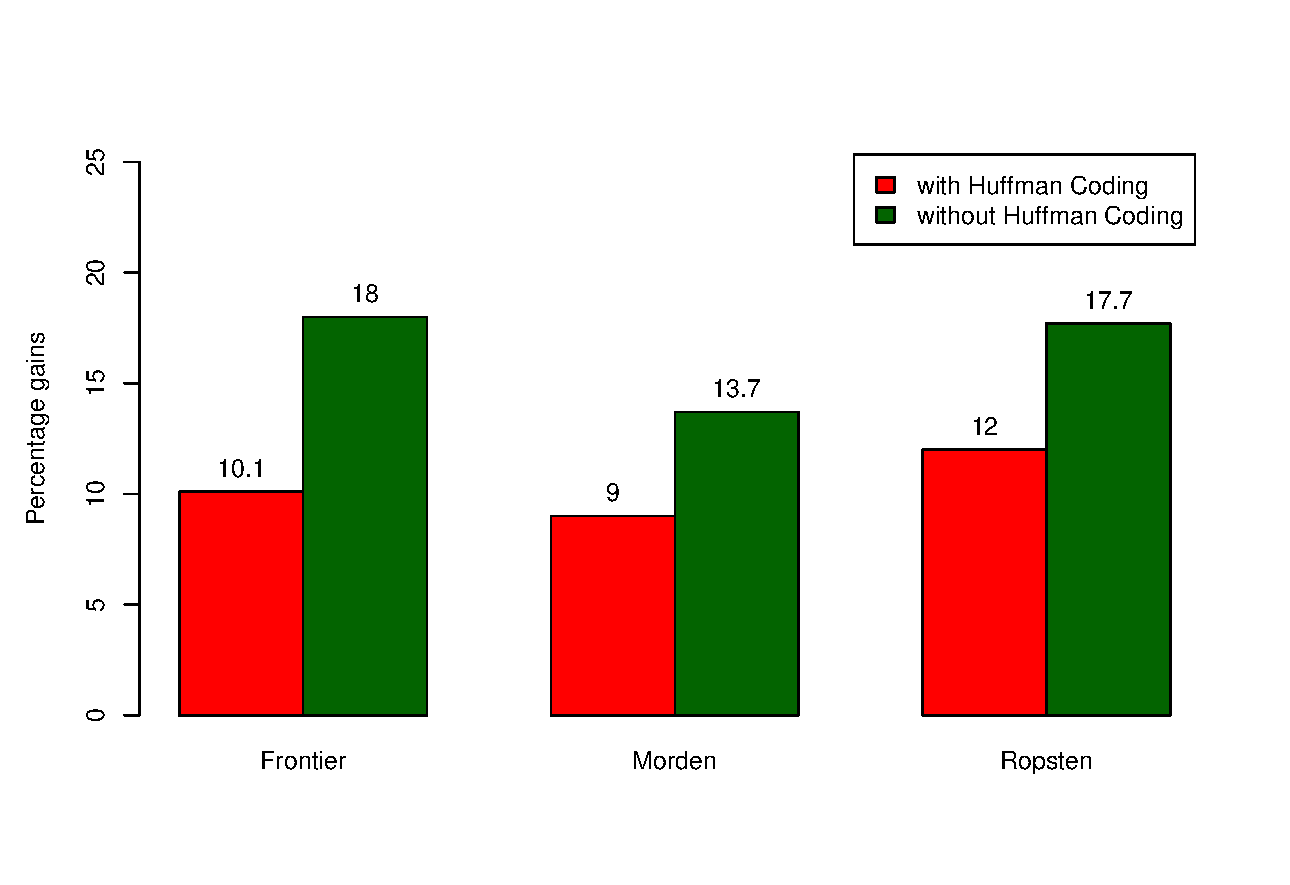
\includegraphics[scale=0.45]{plots/gzip.eps}
	\caption{Additional compression gains (\%) using gzip}
	\label{fig:gzip}
\end{figure}

\begin{figure}[H]
\begin{subfigure}{0.45\textwidth}
	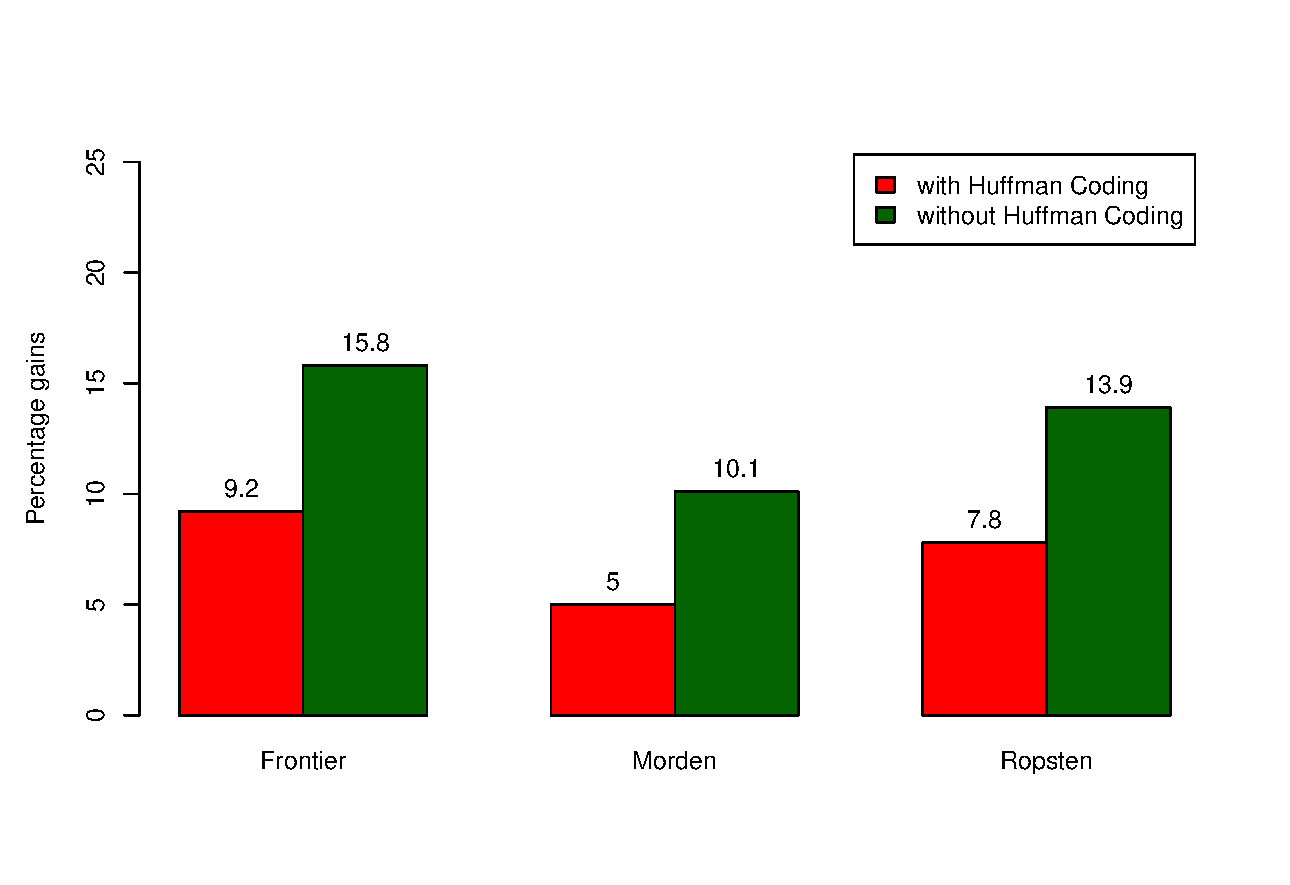
\includegraphics[width=\textwidth]{plots/bzip2.eps}
	\caption{Additional compression gains (\%) using bzip2}
	\label{fig:bzip2}
\end{subfigure}
\begin{subfigure}{0.45\textwidth}
	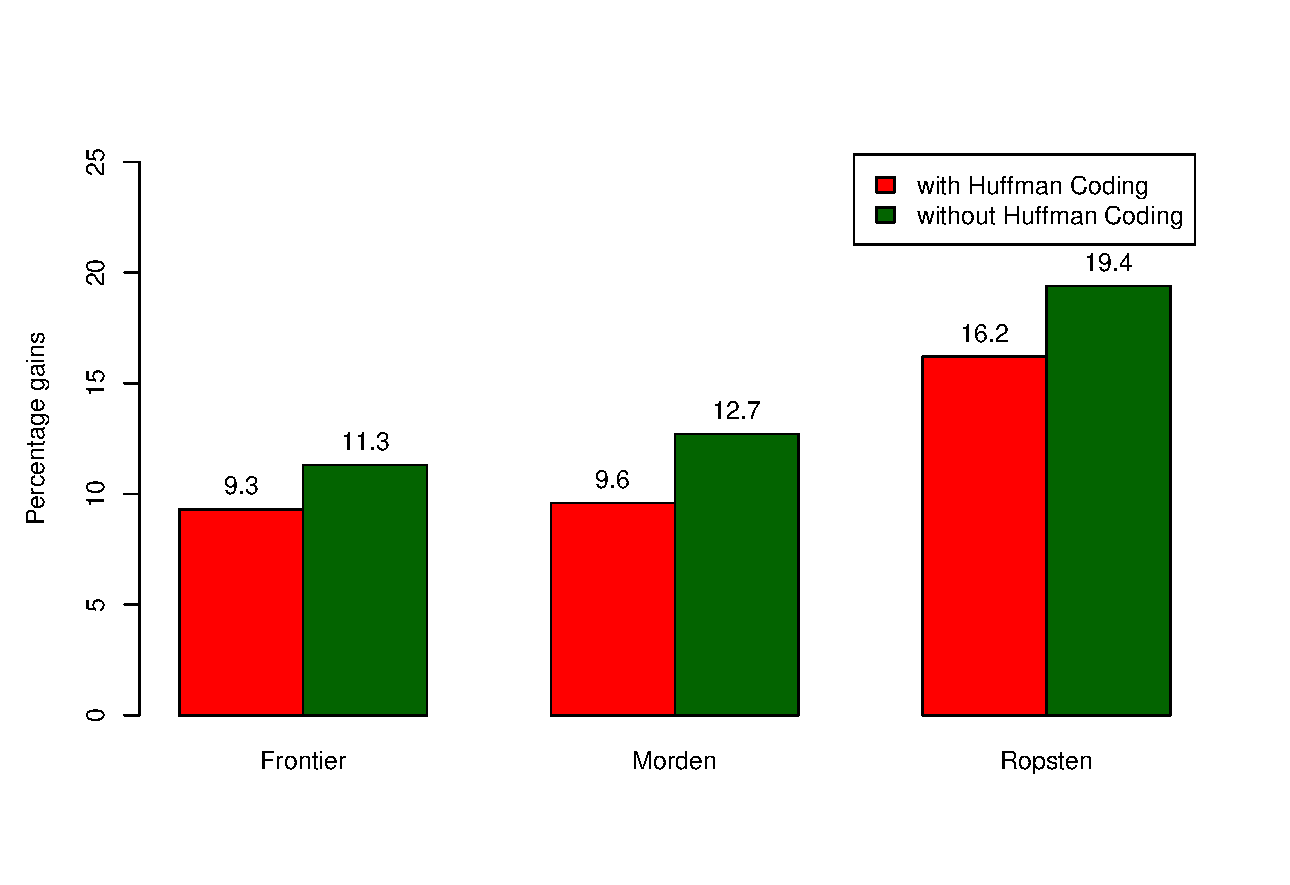
\includegraphics[width=\textwidth]{plots/xz.eps}
	\caption{Additional compression gains (\%) using xz}
	\label{fig:xz}
\end{subfigure}
\caption{ }
\end{figure}
We summarize the additional compression gains for each compression scheme in \autoref{fig:gzip}, \autoref{fig:bzip2} and \autoref{fig:xz}.
As we can see, the results are encouraging and show room for improvement up to $20\%$ (Ropsten in xz).

To demonstrate the feasibility of our approach, we also measure the time taken for compression. 
For brevity, we only present the values for compressing Morden blockchain.
The runtime performance of our tool is proportional to the total number of blocks and transactions. 
To generate the custom format without Huffman encoding, it takes about 150 seconds to generate the custom format and with Huffman encoding it takes about 250 seconds. 



\begin{table}[H]
	\centering
	\begin{tabular}{>{\bfseries}c | p{3cm} | p{3cm}} 
	Program & {Original Compression Time} & {Compression Time using our custom format} \\
	\hline
	gzip & 220  & 71 \\
	bzip2 & 360  & 245\\
	xz & 1340 & 520 \\
	\end{tabular}
	\caption{Compression time in seconds}
	\label{tab:comptime}
\end{table}
\autoref{tab:comptime} compares the time taken to compress the binaries before and after applying our technique. As expected, it is less for binaries that are in custom format. 
To make a fair comparison, we should also include the time taken to create the custom format i.e., 150 and 250 seconds depending on whether Huffman encoding is turned on.
It is worth noting that our tool is a prototype and is not optimized for runtime performance. 
Yet, the performance is comparable. 
In fact, it outperforms in the case of xz which is encouraging.
\begin{figure}[H]
	\centering
	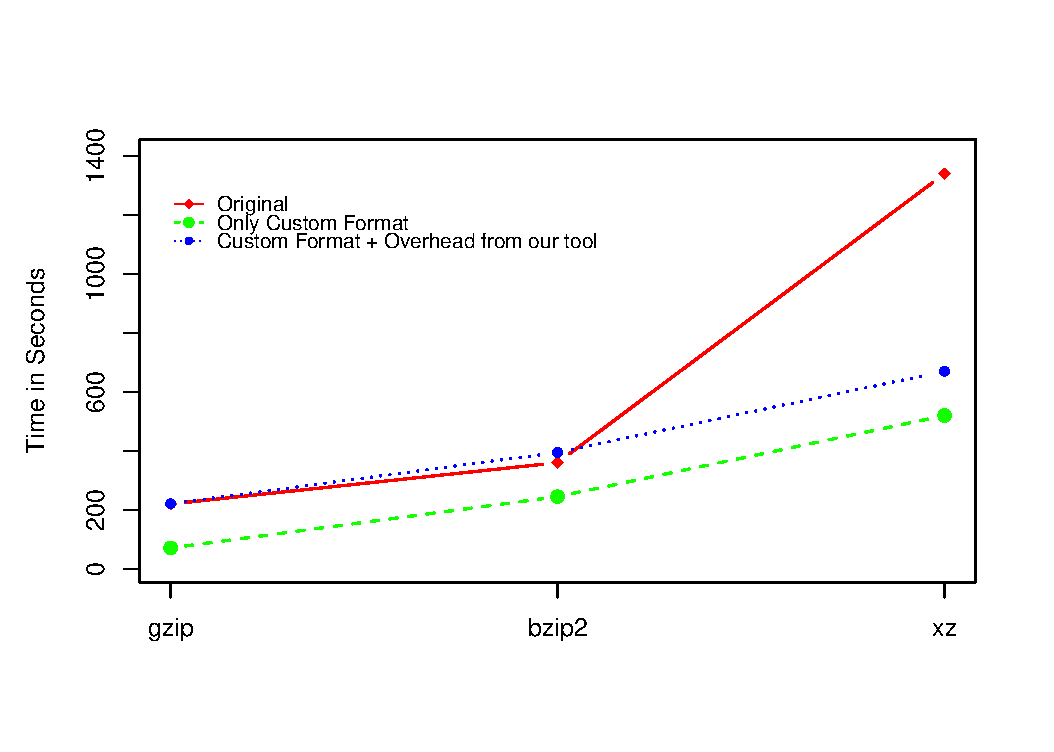
\includegraphics[width=0.5\textwidth, scale=0.5]{plots/time.eps}
	\caption{Compression time in seconds}
	\label{fig:comptime}
\end{figure}
\autoref{fig:comptime} shows the compression time for the original and custom formatted blockchains using gzip, bzip2 and xz.
The solid red line shows the time taken to compress the original blockchain while 
dotted green and blue lines show the same with and without our tool
overheads for custom formatted blockchain. 
As can be seen, initially, the blue line follows the red line closely
but shows a huge difference for the `xz' point.
In the case of xz, the total compression time (including the overhead) is about half the original one, which itself is a significant contribution, considering that xz gives the best compression savings among the three.



\section{Discussion}\label{sec:discuss}
Discuss our results here


\section{Related Work} \label{sec:related}
We identify two broad areas of related work.

\paragraph{Blockchain Compression}
Though blockchain scalability is a well-known problem in the cryptocurrency community,
surprisingly very little effort is seen towards compressing the size of the blockchain.
Much effort is focused on changing the underlying protocol so that clients
do not have to store and process the full blockchain to verify the transactions~\cite{lightclient, ultimate}.
By contrast, we focus on compressing the blockchain without changing the underlying protocol.
We aren't aware of any special techniques for that are already implemented in this direction.


\paragraph{Bytecode Compression}
There are existing solutions to bytecode compression, most of which designed for JVM bytecode.
EVM bytecode and JVM bytecode are very similar and thus many of the proposed compression techniques for JVM bytecode
will also work in the context of EVM bytecode.

F. Aslam et al.~\cite{aslam2010} proposed a JVM compaction mechanism to overcome resource constraints in embedded systems.
It utilizes unused opcode encoding space to extend the JVM bytecode with new instructions that represent bundles of
instructions that often appear together, or common opcode-operand pairs within the same instruction.
The compaction scheme is different from traditional compression in that it does not require decompression before executing,
but requires an augmented JVM instead. It was shown that bytecode compaction can reduce code size for up to 58\%.

M. Latendresse and M. Feeley~\cite{marc2003} applied Huffman encoding to JVM bytecode, and designed interpreters that
can execute bytecode in compressed form by decompressing on-the-fly.
The system focused heavily on performance, which is not critical for Ethereum smart contracts.

Both~\cite{aslam2010} and~\cite{marc2003} feature compressed bytecode that can be executed directly, without decompressing
the entire bytecode block first. It is because these systems were designed for resource-constrained embedded systems.
Ethereum full nodes, however, are usually powerful computers that also need to carry out resource intensive tasks such as
proof-of-work calculation (mining) and/or transaction validation. This requirement of direct execution in compressed form,
therefore, may not be necessary.

W. S. Evans and C. W. Fraser~\cite{evans2003} proposed a grammar-based compression mechanism for identifying patterns in
interpreted bytecode sequences.
Similar to~\cite{aslam2010}, identified patterns are replaced with new instructions to achieve compression, and the semantics
of these new instruction are stored in the augmented interpreters only. Compared to~\cite{aslam2010}, the techniques for
identifying patterns described here are very similar to Sequitur and much more sophisticated than those in~\cite{aslam2010}.

L. R. Clausen et al.~\cite{clausen2000} proposed yet another pattern-based bytecode compression scheme. The system ``factorizes''
the JVM bytecode program by replacing repetitive bytecode sequences with special ``macro'' instructions. The semantics of the
macro instructions are stored in a separate file and can be loaded to the interpreter. Patterns of recurring bytecode sequences
are identified with a greedy algorithm similar to~\cite{aslam2010}. Results show that this scheme can achieve compression rates
similar to gzip.

Most of the ideas in previous work on JVM bytecode compression are applicable to EVM bytecode. EVM bytecode, however, are
both simpler and more complex at the same time, potentially requiring some special treatment. For example, EVM bytecode deals
with simple global unstructured states and therefore doesn't have special field addressing instructions like JVM does.
This means that operands to EVM bytecode instructions are always data that's being pushed or compared to values stored on
the stack, but not meta-values that have implicit meanings in the interpretation of the program.
Due to the cryptographic nature of Ethereum, however, EVM bytecode might need to deal with operand immediate values that
represent Ethereum addresses, which are long cryptographic hash values and hence not compressible. All bytecode compression
techniques mentioned above treat opcode and operand together during the pattern matching process and therefore would identify
instructions with different operands as different patterns.
We look forward to combining existing bytecode compression approaches as well as incorporating special treatment for EVM
bytecode operands to devise a new compression scheme that's tailored to EVM bytecode.


\section{Future Work and Conclusion}\label{sec:future}
In this project we propose a transformation that rearranges the \eth{} blockchain resulting in about $40\%$ space savings on real blockchain.
We also demonstrate that existing compression programs benefit from the custom format. Additional gains of about $19.4\%$ in the best case and $10\%$ in the worst case are possible.
Our transformation adds a little overhead and 
the resulting runtime performance is comparable with that of gzip and bzip2 thout it outperforms in the case of xz. 
Below, we discuss a few possible future directions of the work.

Ethereum blockchain uses bloom filter to easily search the log entries of all transactions in a block.
Currently, we are only using a variant of run-length encoding to compress the Bloom filter, since it is sparse anyway. 
\citet{mitzenmacher:2001} describe a more sophisticated Bloom filter compression technique by tuning the number of hash functions to be used. 
In future, we plan to use this technique to further reduce the number of bits to be broadcast to full nodes.
In particular, we think that coming up with a different number of hash functions (go-ethereum uses 3 hash functions) can compress the Bloom filter more effectively.

We also plan to focus on improving the runtime performance of our tool for compressing and decompressing the blockchain.
Using techniques for hiding the I/O latencies of file I/O, we can amortize 
the overhead incurred for decompressing the blockchain.




%\section{Backup Plan}\label{sec:backup}
%We plan to tackle the question from both the perspective of the blockchain structure and the EVM bytecode.
If it doesn't work out within the timeframe of the project, we plan to concentrate our effort on the EVM
bytecode compression aspect only.
We have already identified where the bytecode is located in the \eth{} source code, and our approach of
separating opcode and operands should not be too hard to implement.
This is a very concrete part of the project that we are confident that we can finish in time.


%\section{Conclusion} \label{sec:conclusion}

% We recommend abbrvnat bibliography style.

\bibliography{mybib}
\bibliographystyle{abbrvnat}

\appendix

\end{document}

%                       Revision History
%                       -------- -------
%  Date         Person  Ver.    Change
%  ----         ------  ----    ------

%  2013.06.29   TU      0.1--4  comments on permission/copyright notices

,
